%
% main.tex -- Paper zum Thema <autotune>
%
% (c) 2023 Florian Baumgartner, OST Ostschweizer Fachhochschule
%
% !TEX root = ../../buch.tex
% !TEX encoding = UTF-8
%
\chapter{Auto-Tune\label{chapter:autotune}}
\kopflinks{Auto-Tune}
\begin{refsection}
\chapterauthor{Florian Baumgartner}

%
% einleitung.tex -- Beispiel-File für die Einleitung
%
% (c) 2023 Dmitry Grigoriev, OST Ostschweizer Fachhochschule
%
% !TEX root = ../../buch.tex
% !TEX encoding = UTF-8
%
\section{Einleitung\label{spektral:section:Einleitung}}
\rhead{Einleitung}

Spektrale Methoden spielen eine wichtige Rolle in der Meteorologie, insbesondere in der Analyse von atmosphärischen Phänomenen und Daten.
Diese Methoden basieren auf der Fourier-Transformation, die es ermöglicht, Signale in den Frequenzbereich zu transformieren und somit ihre spektrale Zusammensetzung zu analysieren.
In der Meteorologie werden spektrale Methoden auf verschiedene Arten angewendet:

\begin{itemize}
\item
\textbf{Spektrale Analyse von Zeitreihen:} Meteorologische Daten, wie Temperatur, Druck, Windgeschwindigkeit usw., werden oft als Zeitreihen erfasst.
Die Fourier-Transformation ermöglicht die Aufschlüsselung dieser Zeitreihen in verschiedene Frequenzkomponenten.
Dies kann hilfreich sein, um periodische Muster oder Trends in den Daten zu identifizieren. 
Zum Beispiel können saisonale Schwankungen in den Temperaturdaten erkannt werden.
\item
\textbf{Wellenanalyse:} Spektrale Methoden werden verwendet, um Wellenphänomene in der Atmosphäre zu analysieren, wie zum Beispiel atmosphärische Schwingungen, Schallwellen, Gezeitenwellen und Rossby-Wellen.
Die Identifizierung von Wellenmustern und -frequenzen hilft bei der Vorhersage von Wetter- und Klimaereignissen.
\item
\textbf{Numerische Wettervorhersage (NWP):} In der numerischen Wettervorhersage werden spektrale Methoden verwendet, um die atmosphärischen Zustandsänderungen im Laufe der Zeit zu simulieren.
Dies geschieht durch die Diskretisierung der atmosphärischen Gleichungen im spektralen Raum und ihre Lösung mithilfe von numerischen Verfahren.
Diese Modelle helfen bei der Vorhersage von Wetterereignissen über verschiedene Zeitskalen.
\item
\textbf{Klimaforschung:} In der Klimaforschung werden spektrale Methoden verwendet, um langfristige klimatische Veränderungen zu analysieren.
\end{itemize}

Diese Anwendungen verdeutlichen, wie spektrale Methoden in der Meteorologie zur Analyse, Modellierung und Vorhersage von atmosphärischen Phänomenen und Prozessen eingesetzt werden können.

Wir werden uns auf die Wellenanalyse und die Numerische Wettervorhersage konzientrieren.
%
% 01_Pitch_Detektion.tex
%
% (c) 2023 Florian Baumgartner, OST Ostschweizer Fachhochschule
%
% !TEX root = ../../buch.tex
% !TEX encoding = UTF-8
%
\section{Pitch-Detektion
\label{autotune:section:pitchDetektion}}
\rhead{Pitch-Detektion}
Bei einer einstimmigen Aufnahme, beispielsweise der menschlichen Stimme oder eines Blasinstruments,
wird die Grundharmonische als Tonhöhe angeschaut.
Es gilt nun, diese zu finden. Es gibt mehrere Möglichkeiten dies umzusetzen.
Im Rahmen dieses Papers werden zwei Methoden verglichen.

\subsection{Short-Time Fourier-Transformation (STFT)
\label{autotune:subsection:shortTimeFourierTransformation}}
Die Short-Time Fourier-Transformation (STFT) ist eine Fourier-Transformation, die auf einem kleinen,
zeitlich begrenzten Ausschnitt eines Signals angewendet wird.
Da es sich sich um einen diskreten Vorgang handelt, wird die STFT beschrieben als
\begin{equation}
    \mathbf{STFT}_x(m, w)
    =
    \sum_{n=-\infty}^{\infty}x(n)\;w(n-m)\;e^{-j\omega n}.
\end{equation}
Dabei definiert $x(n)$ das Signal, $w(n)$ das Fenster und $m$ den Verschiebungsparameter.
Üblicherweise wird ein Fenster der Länge $N$ verwendet, wobei $N$ eine Zweierpotenz ist.
Je länger das Zeitfenster, desto höher ist die physikalische Frequenzauflösung. Jedoch reduziert sich die zeitliche Spektrumabtastung.
Dieser Trade-Off kann gut anhand eines Beispiels gezeigt werden.

\[
    f_s = 44100\;\text{Samples/s} \quad\quad l_w = 23\;\text{ms} \quad\quad L = f_s \cdot l_w = 1014.3 \approx 1024\;\text{Samples}
\]
\[
    \Delta f = \frac{f_s}{L}\approx 43.07\;\text{Hz}
\]

Es fällt auf, dass mit einer Fensterlänge von 23\;ms die Frequenzauflösung bei nur 43.07\;Hz liegt.
Da einzelne Töne jedoch nur wenige Hertz auseinander liegen, können diese nur ungenau voneinander unterschieden werden.
Schnelle Melodien verhindern das Verlängern der Fensterzeit, da sonst mehrere Töne auf ein Segment fallen und nicht mehr identifiziert werden können.

Bei einer Fensterlänge von 23\;ms wird das Spektrum also ca. 43 mal pro Sekunde abgetastet.
Wie in Abbildung \ref{autotune:fig:pitchDetektionSTFT} zu sehen ist, können somit auch schnelle Tonhöhenänderung erkannt werden.

\begin{figure}
	\centering
	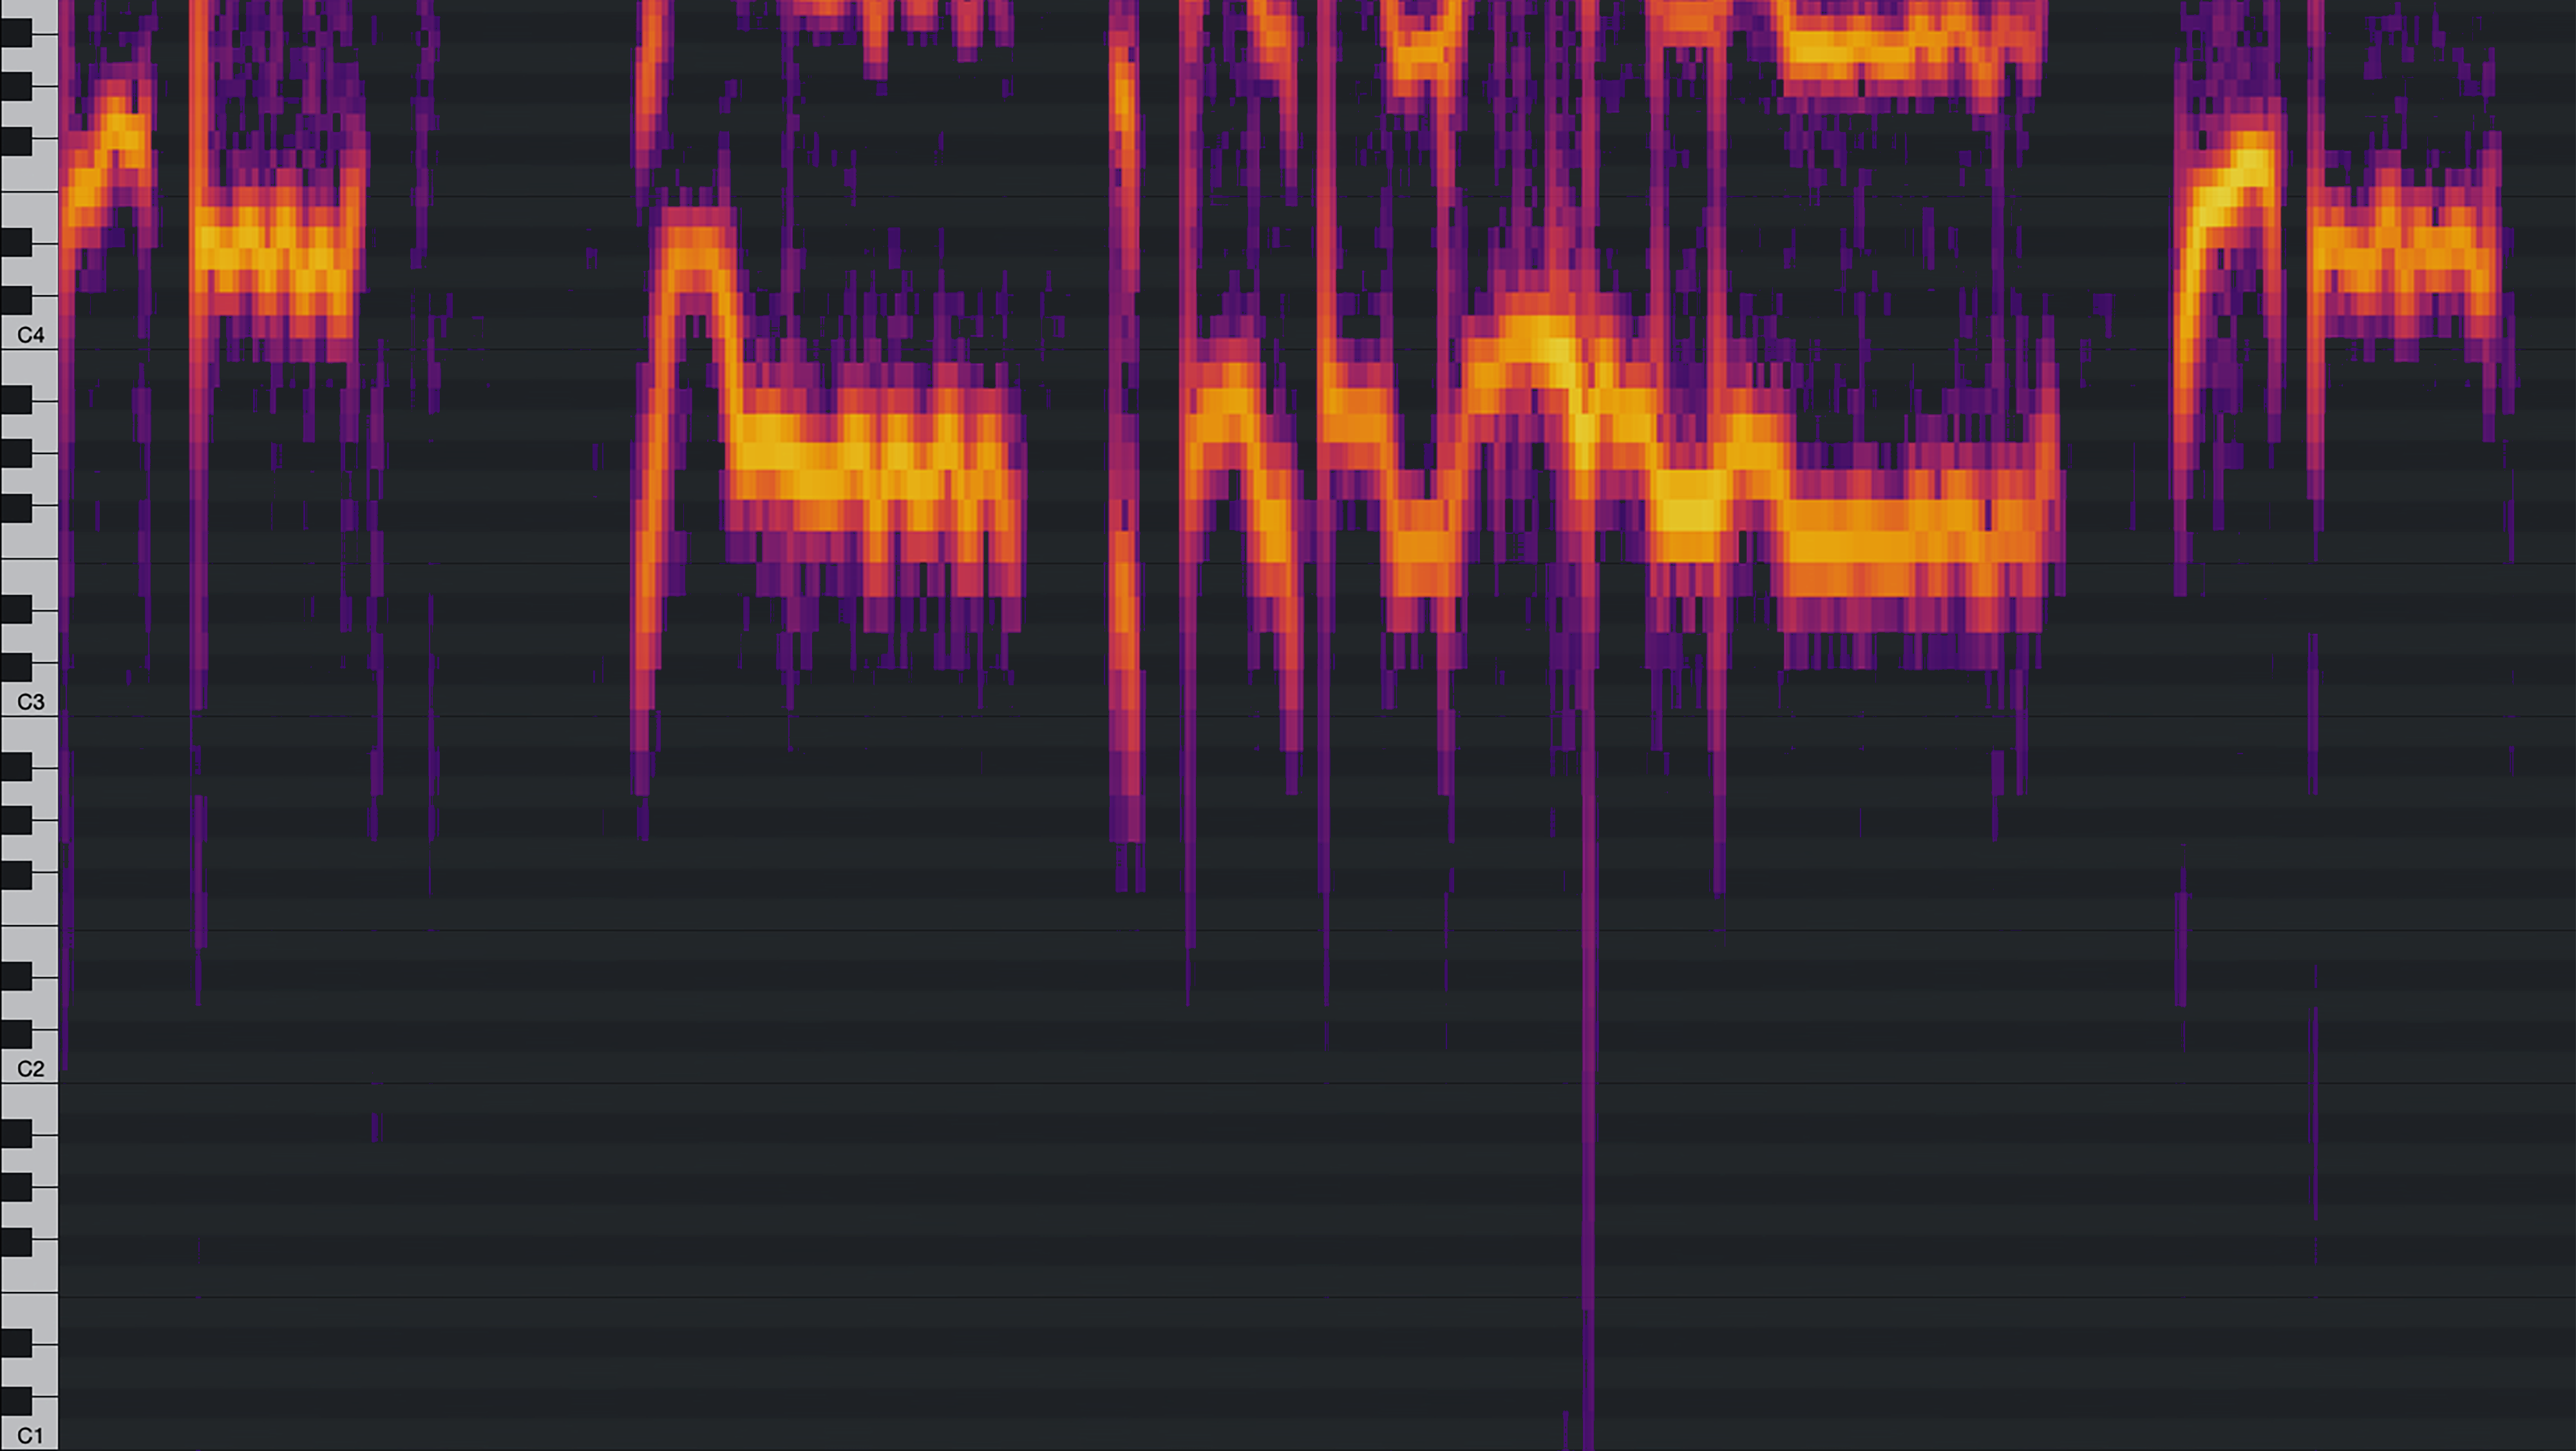
\includegraphics[width=\textwidth]{papers/autotune/images/Pianoscale_Example_Detuned_STFT.png}
	\caption{Pitch-Detektion mit STFT (Fensterlänge von 23\;ms).}
    \label{autotune:fig:pitchDetektionSTFT}
\end{figure}

Diese spektrale Darstellungsweise wird auch als Sonogramm bezeichnet. Mehr dazu im Kapitel \ref{chapter:sonogramm}.


Das konkrete bestimmen der Tonhöhe innerhalb eines Fensters kann auf verschiedene Arten umgesetzt werden.
Eine Möglichkeit ist das Bestimmen der Grundharmonischen durch das Finden des Maximums im Spektrum (Peak-Detektor).
Mathematisch ausgedrückt als

\begin{equation}
    f_{\text{pitch}}
    =
    \arg\max_{f}{\left | \; \mathbf{STFT}_x(m, w) \; \right |}^2.
\end{equation}


\subsection{Cumulative Mean Normalized Difference Function (CMNDF)
\label{autotune:subsection:cumultativeMeanNormalizedDifferenceFunction}}
Eine weitere Methode zur Tonhöhenbestimmung ist die Cumulative Mean Normalized Difference Function (CMNDF).
Diese Methode basiert auf der Auto-Korrelation des Signals welche definiert ist als

\begin{equation}
    \mathbf{ACF}(\tau, t)
    =
    \sum_{i=t}^{t+W}f(x_i)\cdot f(x_i+\tau).
\end{equation}

Dabei ist $\tau$ die Verzögerung innerhalb des Fensters und $W$ die Fensterlänge.
Daraus folgend kann die Quadrierte Differenz Funktion $\mathbf{DF}$ hergeleitet werden als

\begin{equation}
    \begin{aligned}
        \mathbf{DF}(\tau,t)
        &= \sum_{i=t}^{t+W}\left(f(x_i)-f(x_i+\tau)\right)^2 \\
        &= \sum_{i=t}^{t+W}\left(f(x_i)^2+f(x_i+\tau)^2-2 \cdot f(x_i) \cdot f(x_i + \tau)\right) \\
        &= \mathbf{ACF}(0,t)+\mathbf{ACF}(0,t+\tau)-2\cdot \mathbf{ACF}(\tau,t).
    \end{aligned}
\end{equation}

Die $\mathbf{DF}$ liefert den normalisierten absoluten \glqq Überlagerungsfehler\grqq\ zum Zeitpunkt $t$ des Signals $f$ und einer um $\tau$ verzögerten Version von $f$.
Bei $\tau=0$ ist der Überlagerungsfehler 0, da das Signal mit sich selbst verglichen wird.
Die $\mathbf{CMNDF}$ ist definiert als 

\begin{equation}
    \mathbf{CMNDF}(\tau,t)
    =
    \left\{
        \;\begin{array}{ll} 0 & \tau=0 \\
        \tau \cdot \frac{\mathbf{DF}(\tau,t)}{\sum\nolimits_{j=1}^{\tau} \mathbf{DF}(j,t)} & \tau > 0 \end{array}
    \right\}.
\end{equation}


Gesucht wird nun das erste lokale Minimum der CMNDF.
Dieses Minimum entspricht der Periodendauer der Grundharmonischen.
Grafisch dargestellt ist dies in Abbildung \ref{autotune:fig:cmndfMinimum}.

\begin{figure}
	\centering
	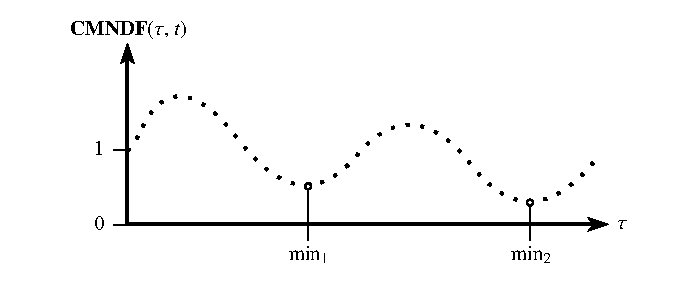
\includegraphics[width=0.8\textwidth]{papers/autotune/images/CMNDF_Minimum.pdf}
	\caption{Finden der lokalen Minima von CMNDF.}
    \label{autotune:fig:cmndfMinimum}
\end{figure}


Es fällt auf, dass die CMNDF mehrere lokale Minima aufweist.
Diese entsprechen den höhren Harmonischen und sind nicht von Interesse.
In der Praxis erweist es sich zum Teil als schwierig, das erste lokale Minimum zu finden.
Oft wird deshalb ein Schwellwert definiert.
An der Stelle wo die CMNDF diesen Schwellwert unterschreitet, wird das Minimum definiert.
Die Tonhöhe kann nun bestimmt werden als

\begin{equation}
    f_{pitch}
    =
    \frac{1}{min_1}.
\end{equation}


Die CMNDF ist im Vergleich zur STFT wesentlich effizienter und liefert sowohl eine hohe Frequenzauflösung als auch eine hohe zeitliche Auflösung.
Dies ist in Abbildung \ref{autotune:fig:pitchDetektionCMNDF} gut ersichtlich.

\begin{figure}
	\centering
	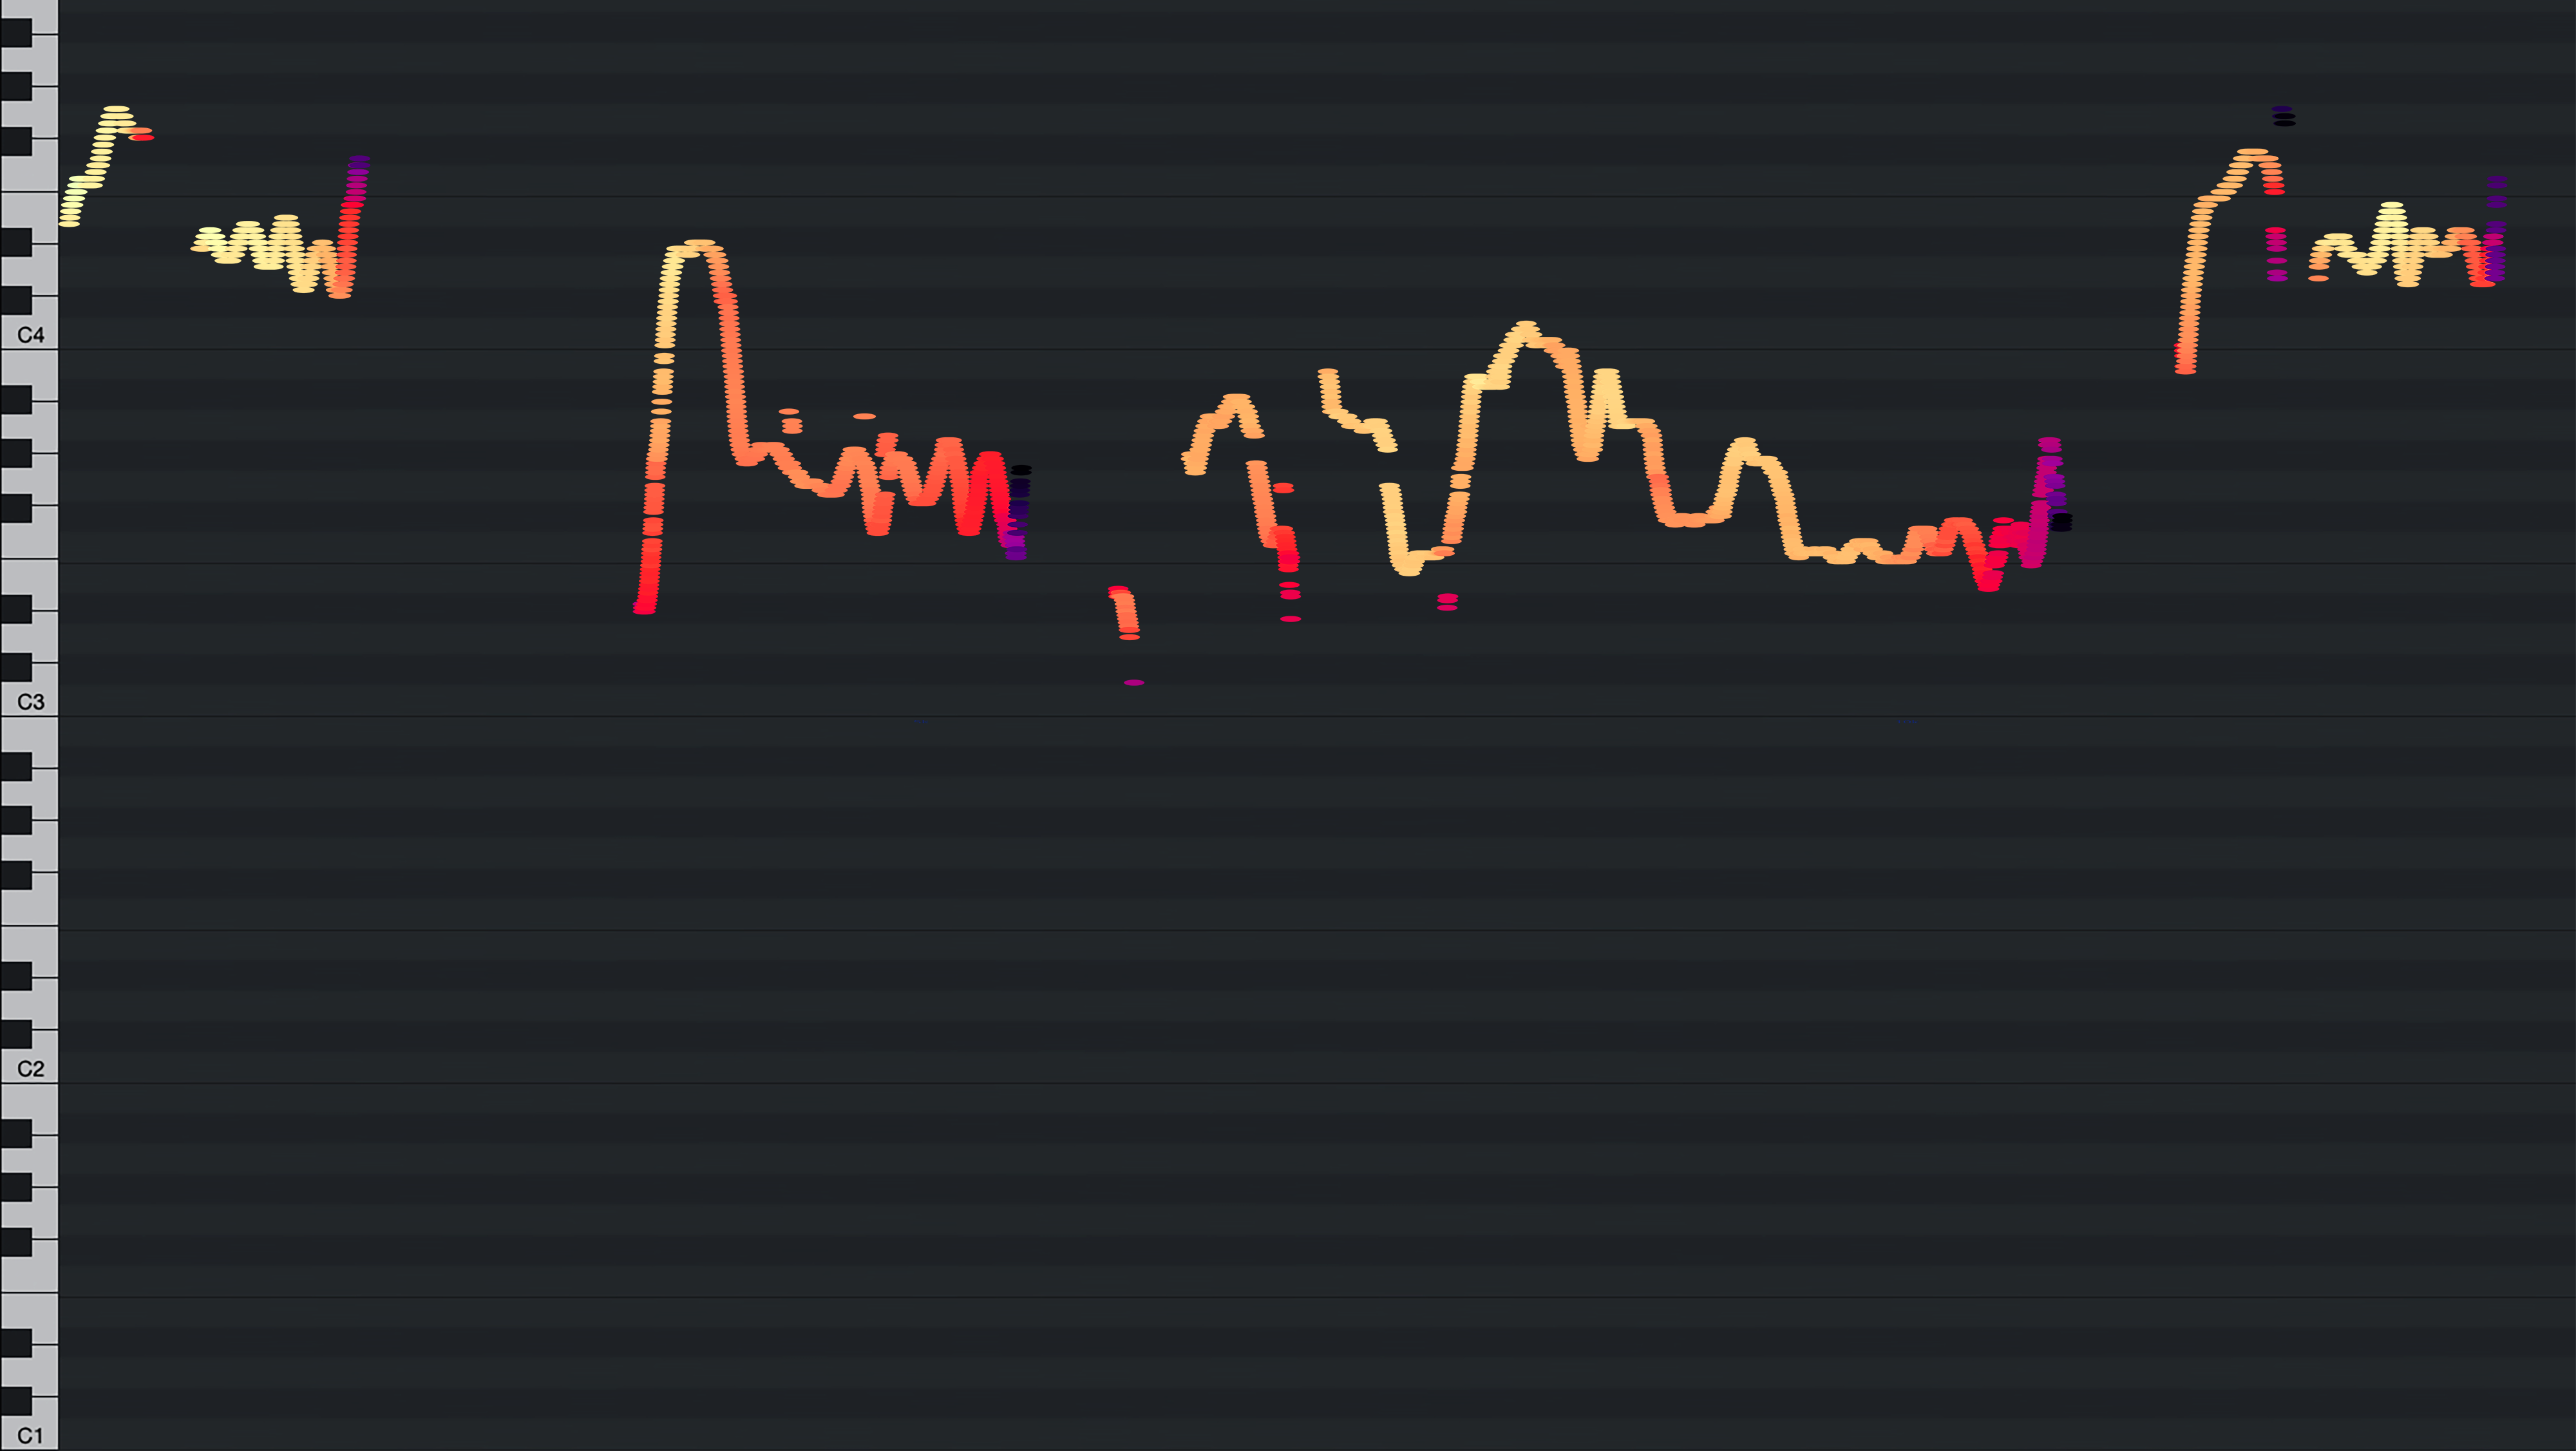
\includegraphics[width=\textwidth]{papers/autotune/images/Pianoscale_Example_Detuned_CMNDF.png}
	\caption{Pitch-Detektion mit CMNDF.}
    \label{autotune:fig:pitchDetektionCMNDF}
\end{figure}


Es zeigt sich, dass kommerzielle Software-Tools mit grosser Wahrscheinlichkeit die CMNDF-Methode verwenden.
So stimmen die eigens mittels CMNDF berechneten Tonhöhen mit denjenigen der kommerziellen Software \textit{Steinberg Cubase 12 Pro VariAudio} überein,
welche als Referenz verwendet wurde. Dies ist dargestellt in Abbildung \ref{autotune:fig:pitchDetektionCMNDFReference}.

\begin{figure}
	\centering
	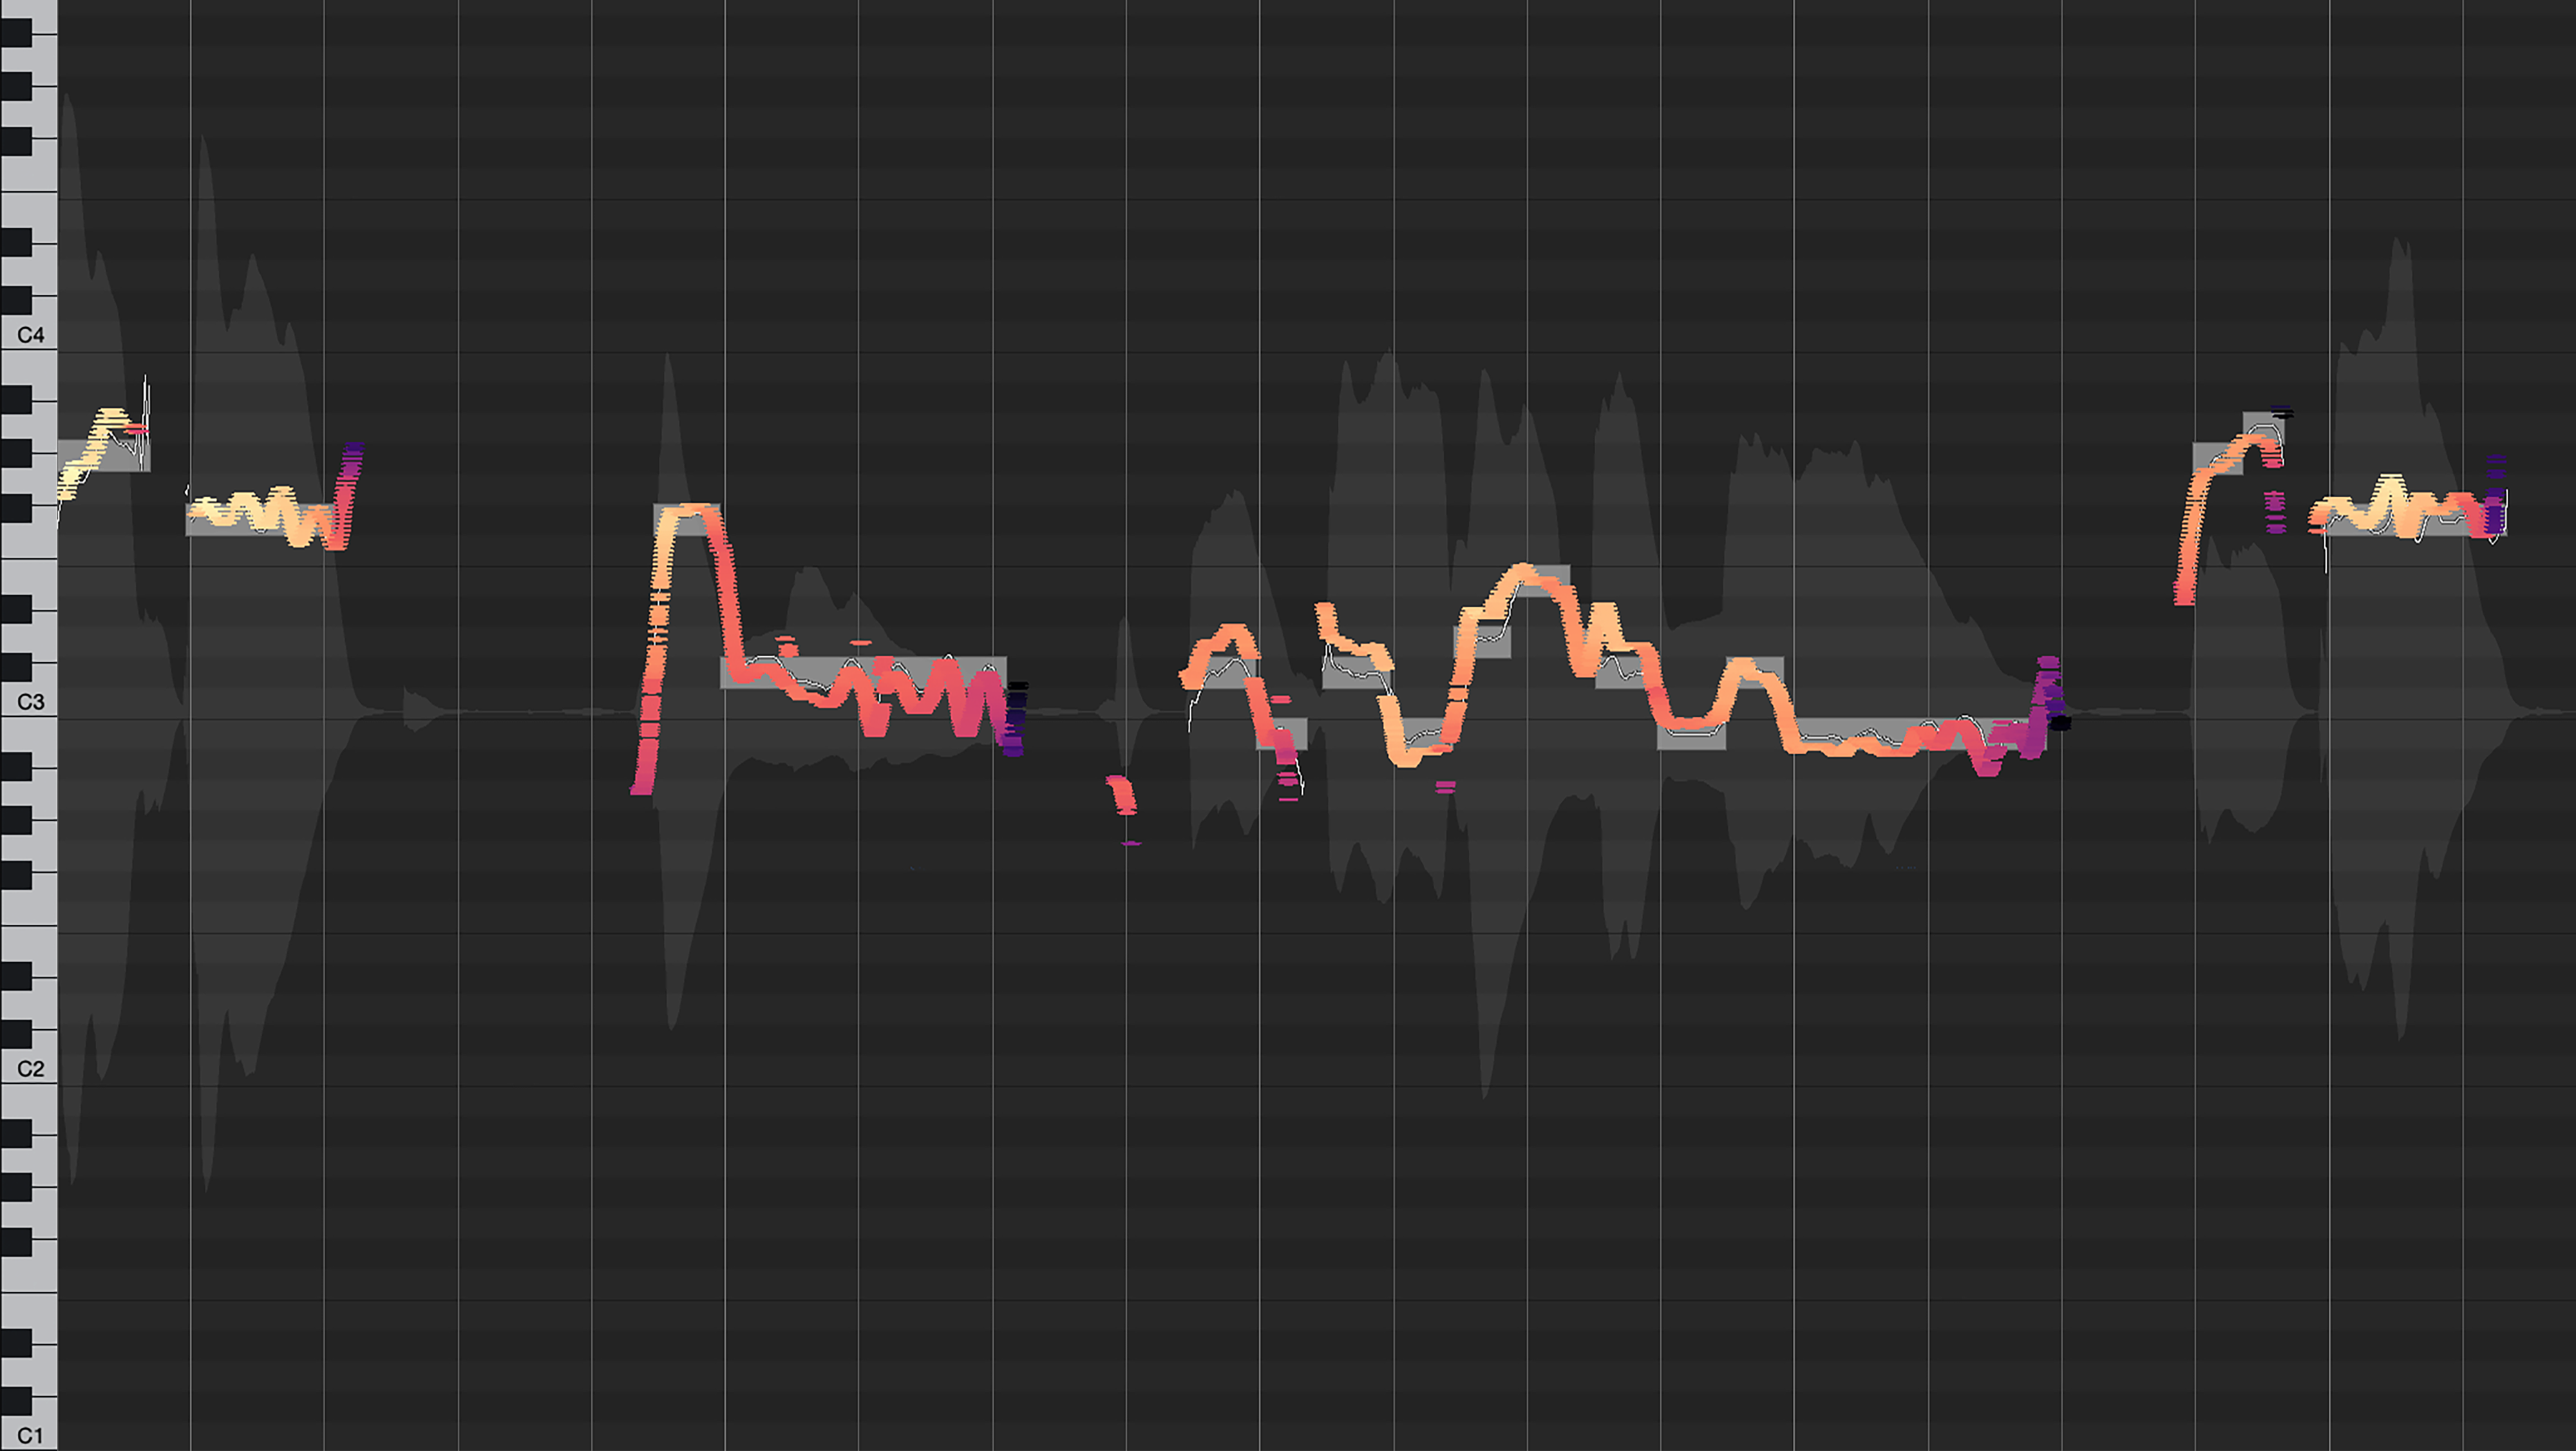
\includegraphics[width=\textwidth]{papers/autotune/images/Pianoscale_Example_Detuned_CMNDF_Reference.png}
	\caption{Vergleich der Tonhöhenbestimmung mit CMNDF und kommerzieller Auto-Tune Software (Steinberg Cubase 12 Pro VariAudio).}
    \label{autotune:fig:pitchDetektionCMNDFReference}
\end{figure}

%
% 02_Pitch_Tonsystem_und_Stimmung.tex
%
% (c) 2023 Florian Baumgartner, OST Ostschweizer Fachhochschule
%
% !TEX root = ../../buch.tex
% !TEX encoding = UTF-8
%
\section{Tonsystem und Stimmung
\label{autotune:section:tonsystemUndStimmung}}
\rhead{Tonsystem und Stimmung}
In der westlichen Musik wird das Tonsystem in 12 (Halb)-Töne pro Oktave unterteilt (chromatische Skala).
Dabei gibt es verschiedene Möglichkeiten wie diese zueinander gestimmt werden, also wie sich die Anordnung der Töne unterscheiden.

Als Kammerton, auch Normalstimmton genannt, wird der Ton bezeichnet auf den sich alle Instrumente einstellen.
International hat sich der Kammerton A4 mit einer Frequenz von 440\;Hz durchgesetzt.
Jedoch gibt Länder welche andere Frequenzen verwenden, so ist in der Schweiz der Kammerton A4 mit 442\;Hz üblich.
Im Rahmen dieser Arbeit wird der Kammerton A4 definiert als 
\begin{equation}
    f_{A4}
    =
    440\;\text{Hz}.
\end{equation}

\subsection{Gleichstufige Stimmung
\label{autotune:subsection:gleichstuffigeStimmung}}
Die gleichstufige Stimmung ist das meist verbreitetet Stimmungssystem in der westlichen Musik, insbesondere bei Tasteninstrumenten.
Es ist ein System, bei dem die Oktave in zwölf Halbtöne aufgeteilt ist,
wobei das Frequenzverhältnis zwischen jedem Paar aufeinanderfolgender Töne gleich ist.
Dieses Verhältnis ist die zwölfte Wurzel aus zwei ($\approx 1.05946$) und berechnet sich als

\begin{equation}
    f_n
    =
    \sqrt[12]{2^n} \cdot f_{A4}
    \quad | \quad
    n \in \mathbb{Z}.
\end{equation}

Der Vorteil der gleichstufigen Stimmung ist, dass sie in allen Tonarten gleich funktioniert, was bedeutet,
dass ein Musikstück in jede Tonart transponiert werden kann, ohne dass sich die harmonischen Beziehungen zwischen den Tönen ändern.
Ein Nachteil ist jedoch, dass die Intervalle (ausser Oktaven) nicht völlig rein sind, das heisst,
sie weichen leicht von den einfachen ganzzahligen Frequenzverhältnissen ab, die in der reinen Stimmung verwendet werden.

\subsection{Reine Stimmung
\label{autotune:subsection:reineStimmung}}
Die reine Stimmung, auch bekannt als natürliche oder harmonische Stimmung, ist ein System,
das auf den natürlichen Harmonischen basiert, die in den Schwingungsmustern physikalischer Objekte wie Saiten oder Luftsäulen gefunden werden.
In diesem System werden die Frequenzen der Noten so gewählt, dass sie einfache ganzzahlige Verhältnisse zueinander haben.
Zum Beispiel beträgt das Verhältnis der Frequenzen zweier Töne in einer reinen Quinte 3:2, und in einer reinen Quarte 4:3.
Dies führt zu besonders harmonisch klingenden Intervallen ohne stark bemerkbare Schwebungen.
Allerdings bringt die reine Stimmung einige Probleme mit sich.
Während sie innerhalb einer einzelnen Tonart sehr gut funktioniert, führt sie zu Unstimmigkeiten,
wenn man versucht, zwischen verschiedenen Tonarten zu wechseln.
Deshalb ist die reine Stimmung in der Praxis eher auf Streich- und Blasinstrumente beschränkt,
bei denen die Musiker die Intonation von Noten anpassen können.

In der Tabelle \ref{autotune:table:stimmung} werden die Frequenzen der Töne mit reiner Stimmung verglichen mit der gleichstufigen Stimmung.

\begin{table}[htb]
    \begin{tabular}{ccrlrlll}\toprule
    \begin{tabular}[c]{@{}c@{}}$Tonname$\\ $(gleich)$\end{tabular}   & \begin{tabular}[c]{@{}c@{}}$Tonname$\\ $(rein)$\end{tabular}   & $f_{gleich}$                    & $(Hz)$             & $f_{rein}$                    & $(Hz)$                 & $\Delta{f}\;(Hz)$ & $Abweichung$  \\\midrule
    a                                                                & a                                                              & $\sqrt[12]{2^{ 0}}\cdot f_{A4}$ & $=\textbf{440.00}$ & $\sfrac{1}{1}  \cdot f_{A4}$  & $=\textbf{440.00}$     & $0.00$            & $ 0.00\;\%$   \\
    ais/b                                                            & b                                                              & $\sqrt[12]{2^{ 1}}\cdot f_{A4}$ & $\approx 469.16$   & $\sfrac{16}{15}\cdot f_{A4}$  & $= 469.\overline{33}$  & $3.17$            & $11.73\;\%$   \\
    h                                                                & h                                                              & $\sqrt[12]{2^{ 2}}\cdot f_{A4}$ & $\approx 493.88$   & $\sfrac{9}{8}  \cdot f_{A4}$  & $= 495.00$             & $1.12$            & $ 1.96\;\%$   \\
    c                                                                & c                                                              & $\sqrt[12]{2^{ 3}}\cdot f_{A4}$ & $\approx 523.25$   & $\sfrac{6}{5}  \cdot f_{A4}$  & $= 528.00$             & $4.75$            & $ 5.21\;\%$   \\
    cis/des                                                          & des                                                            & $\sqrt[12]{2^{ 4}}\cdot f_{A4}$ & $\approx 554.37$   & $\sfrac{5}{4}  \cdot f_{A4}$  & $= 550.60$             & $4.37$            & $ 3.42\;\%$   \\
    d                                                                & d                                                              & $\sqrt[12]{2^{ 5}}\cdot f_{A4}$ & $\approx 587.33$   & $\sfrac{4}{3}  \cdot f_{A4}$  & $= 586.\overline{66}$  & $0.66$            & $ 0.39\;\%$   \\
    dis/es                                                           & es                                                             & $\sqrt[12]{2^{ 6}}\cdot f_{A4}$ & $\approx 622.25$   & $\sfrac{45}{32}\cdot f_{A4}$  & $= 618.75$             & $3.50$            & $ 1.63\;\%$   \\
    e                                                                & e                                                              & $\sqrt[12]{2^{ 7}}\cdot f_{A4}$ & $\approx 659.26$   & $\sfrac{3}{2}  \cdot f_{A4}$  & $= 660.00$             & $0.74$            & $ 0.28\;\%$   \\
    f                                                                & f                                                              & $\sqrt[12]{2^{ 8}}\cdot f_{A4}$ & $\approx 698.46$   & $\sfrac{8}{5}  \cdot f_{A4}$  & $= 704.00$             & $5.54$            & $ 1.71\;\%$   \\
    fis/ges                                                          & fis                                                            & $\sqrt[12]{2^{ 9}}\cdot f_{A4}$ & $\approx 739.99$   & $\sfrac{5}{3}  \cdot f_{A4}$  & $= 733.\overline{33}$  & $6.66$            & $ 1.74\;\%$   \\
    g                                                                & g                                                              & $\sqrt[12]{2^{10}}\cdot f_{A4}$ & $\approx 783.99$   & $\sfrac{9}{5}  \cdot f_{A4}$  & $= 792.00$             & $8.01$            & $ 1.76\;\%$   \\
    gis/as                                                           & as                                                             & $\sqrt[12]{2^{12}}\cdot f_{A4}$ & $\approx 830.61$   & $\sfrac{15}{8} \cdot f_{A4}$  & $= 825.00$             & $5.61$            & $ 1.07\;\%$   \\
    a                                                                & a                                                              & $\sqrt[12]{2^{12}}\cdot f_{A4}$ & $=880.00$          & $\sfrac{2}{1}  \cdot f_{A4}$  & $= 880.00$             & $0.00$            & $ 0.00\;\%$   \\\bottomrule
    \end{tabular}
    \caption{Vergleich von Frequenzen der Töne mit reiner und gleichstufiger Stimmung.}
    \label{autotune:table:stimmung}
\end{table}

Es zeigt sich, dass teilweise grosse Abweichungen zwischen den Tönen der reiner und gleichstufiger Stimmung bestehen.
In der gleichstufigen Stimmung kommt es beim Spielen von Kadenzen (z.B. Akkorden) zu Schwebungen.
Dies kann gut anhand eines Beispiels, der c-g Quinte, gezeigt werden. Die Schwebung berechnet sich als

\begin{equation}
    \frac{f_{G4}}{f_{C4}}
    =
    \frac{2^{\frac{10}{12}}\cdot f_{A4}}{2^{\frac{3}{12}}\cdot f_{A4}}
    =
    2^{\frac{7}{12}}
    \approx
    1.4983\;.
\end{equation}

% TODO: Wie gross ist die Schwebung in Hz?


%
% 03_Pitch_Korrektur.tex
%
% (c) 2023 Florian Baumgartner, OST Ostschweizer Fachhochschule
%
% !TEX root = ../../buch.tex
% !TEX encoding = UTF-8
%

\section{Pitch-Korrektur
\label{autotune:section:pitchKorrektur}}
\rhead{Pitch-Korrektur}
Das Ändern der Tonhöhe eines Audiosignals ist keine triviale Aufgabe.
Grundsätzlich ist der Zeit- und Frequenzbereich eines Signals über die Fourier-Transformation miteinander verbunden und kann nicht unabhängig voneinander manipuliert werden.
Dies zeigt der Audruck 
\begin{equation}
    f(t)  \; \laplace \; F(\omega).
\end{equation}
Falls beispielsweise die Tonhöhe eines Audiosignals erhöht werden soll, muss das Audiosignal \glqq schneller\grqq\ abgespielt werden, ähnlich wie bei einer Schallplatte.
Diese Zeitstreckung gillt es jedoch zu vermeiden, da sonst die Dauer der Noten und damit die gesamte Länge der Aufnahme verändert wird.
Algorithmen die die Tonhöhe unabhängig von der Dauer des Audiosignals verändern können, fallen unter den Begriff \textit{Dynamic Time Warping} (DTW).
In der Praxis gibt es eine Vielzahl von Methoden, die sich in ihrer Komplexität und Qualität unterscheiden.
Schlussendlich handelt es sich immer um ein Optimierungsproblem, was für jede Anwendung spezifische Lösungen erfordert.
Wichtig zu erwähnen ist, dass es sich bei allen Algorithmen dieser Art um einen nicht-linearen Prozess handelt,
der verlustbehaftete Resultate liefert.
Im Rahmen dieses Papers wird speziell der \emph{Phase Vocoder} betrachtet, da er die Grundlage für die meisten Auto-Tune-Algorithmen bildet.


\subsection{Phase Vocoder
\label{autotune:subsection:phaseVocoder}}
\rhead{Phase Vocoder}
Der Phase Vocoder ist ein Algorithmus,
der es ermöglicht die Tonhöhe eines Audiosignals zu ändern, ohne andere Attribute wie die Dauer oder den Klang des Signals negativ zu beeinflussen.
Im Wesentlichen arbeitet der Phase Vocoder,
indem er ein Audiosignal in eine Reihe von überlappenden Fenstern (Frames) zerlegt und anschliessend mithilfe der Fourier-Transformation in den Frequenzbereich umwandelt.
Die Tonhöhenänderung erfolgt dann durch das Skallieren der Frequenzen in der Fourier-Domäne.
Nachdem das Signal im Frequenzbereich manipuliert wurde,
wird es mithilfe der inversen Fourier-Transformation zurück in den Zeitbereich gewandelt.
Dabei wird speziell darauf geachtet, die Phase zwischen benachbarten Fenstern möglichst exakt zu rekonstruieren,
um hörbare Artefakte zu minimieren (siehe \ref{autotune:subsection:fensterRekonstruktion}).
Die Phasenrekonstruktion ist der wesentliche Bestandteil des Phase Vocoder,
woraus sich auch dessen Name ableitet.


\subsection{Spektrum Manipulation
\label{autotune:subsection:spektrumManipulation}}
Im Frequenzbereich kann die Tonhöhe eines Signals durch eine einfache Multiplikation der Frequenzen mittels konstantem Faktor verändert werden.
Die lineare Skallierung wird ausgedrückt als
\begin{equation}
    Y_n(\omega)
    =
    X_n(\omega \cdot R) \;.
\end{equation}
Dabei ist $X_n(\omega)$ das Frequenzspektrum des $n$-ten Fensters und $R$ der Skalierungsfaktor welcher berechnet wird als
\begin{equation}
    R
    =
    \frac{f_{\text{Ref}}}{{f_{\text{In}}}} \;.
\end{equation}
Wie im Blockschaltbild \ref{autotune:fig:blockschaltbild} erkennbar ist,
stellt $f_{In}$ die gemessene Tonhöhe innerhalb des Fensters dar und $f_{Ref}$ die gewünschte Tonhöhe,
des nächstliegenden Tons aus der Referenz-Tonleiter:
\begin{equation}
    f_{\text{Ref}}
    =
    \arg\min_n \left| f_n - f_{In} \right|
    \quad | \quad
    f_n \in \{ f_{G2}, f_{G\#2}, f_{A2}, \ldots, f_{F\#4}, f_{G4} \} \; .
\end{equation}
Grafisch dargestellt ist diese Skallierung in Abbildung \ref{autotune:fig:spektrumManipulation}.
\begin{figure}
    \centering
    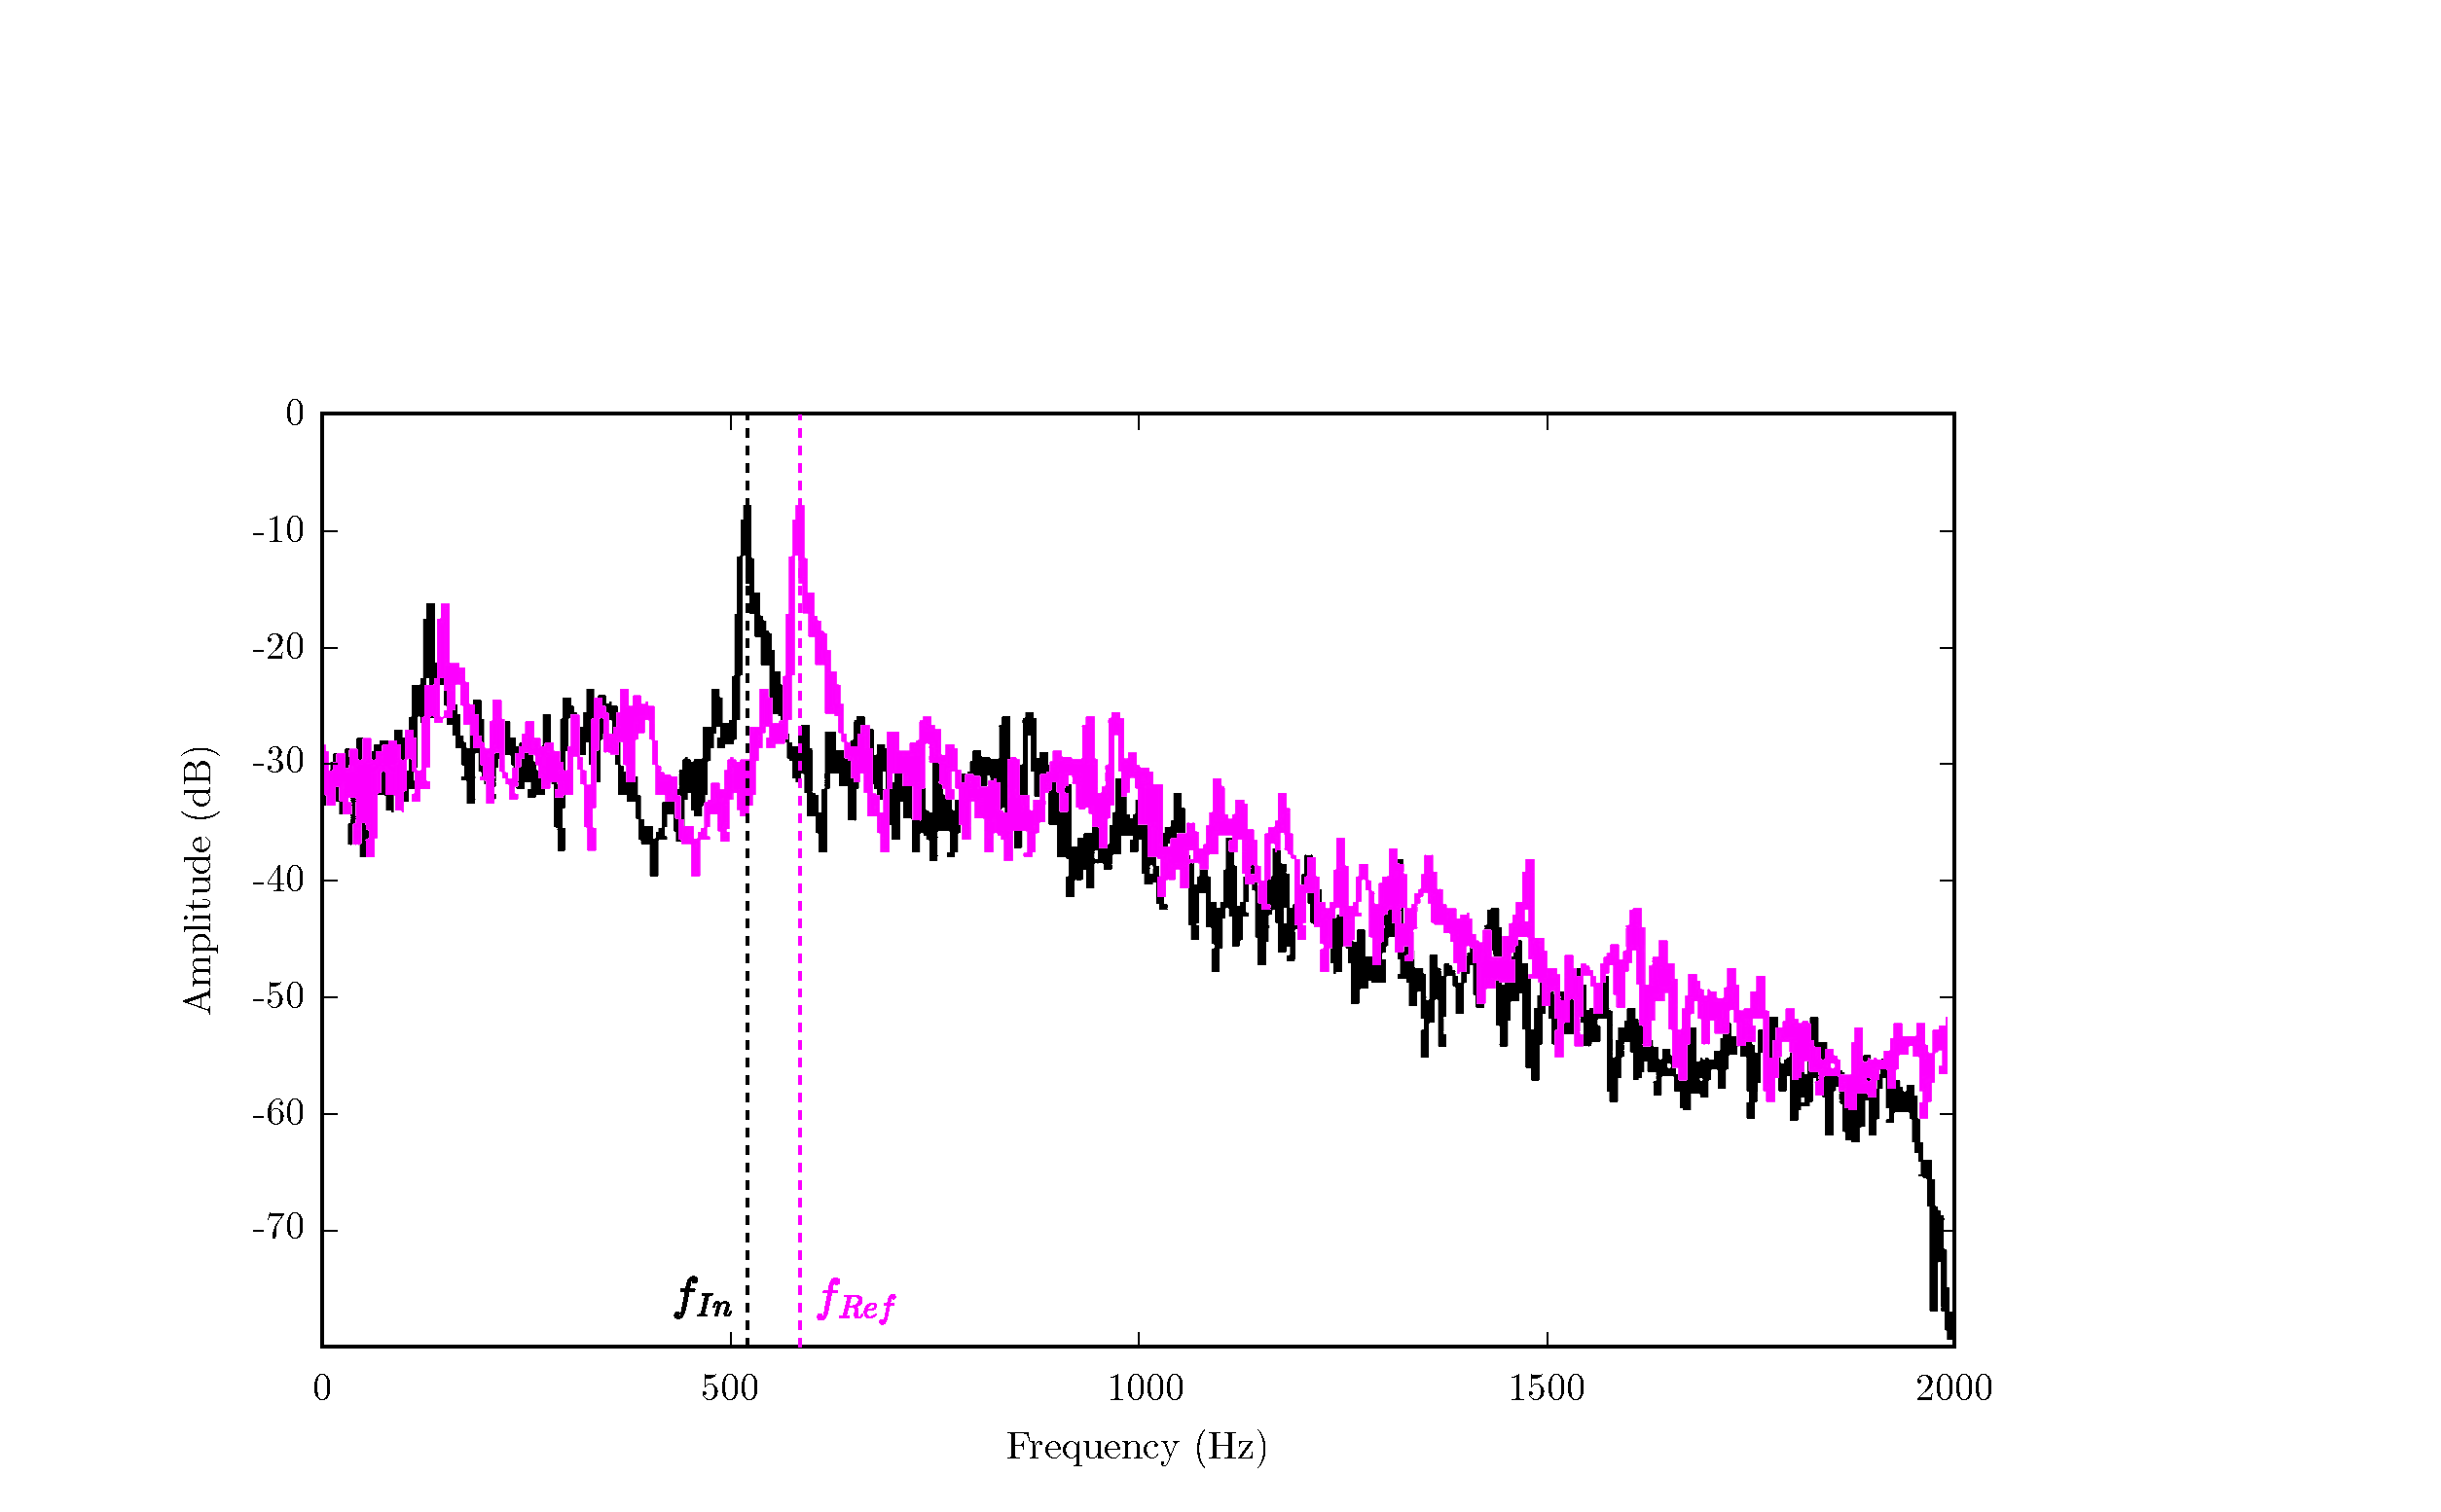
\includegraphics[width=\textwidth]{papers/autotune/images/Spektrum-Manipulation.pdf}
    \caption{Skallierung des Frequenzspektrums}
    \label{autotune:fig:spektrumManipulation}
\end{figure}
Obwohl dieser Ansatz grundsätzlich funktioniert, klingt die resultierende Tonhöhenänderung unnatürlich.
Der entstehende Effekt wird auch als \textit{Chipmunk-Effekt} bezeichnet und ist dafaruf zurückzuführen,
dass die ursprünglichen Formanten des Audiosignals verloren gehen.

%TODO: Add audio example of chipmunk effect

Um den Klangcharakter der menschlichen Stimme beizubehalten,
ist es notwendig das Leistungsdichtespektrum möglichst unverändert zu lassen.
Im nächsten Abschnitt wird erläutert, wie dies erreicht werden kann.


\subsection{Formantenerhaltung
\label{autotune:subsection:formantenErhaltung}}
Formanten sind spezifische Resonanzfrequenzen des menschlichen Vokaltrakts.
Bei der menschlichen Sprachproduktion werden durch die Stimmbänder Schallwellen erzeugt,
die durch den Vokaltrakt (bestehend aus Mund, Nase und Rachen) weiter moduliert werden.
Die Form und Länge des Vokaltrakts bestimmen die Position und Anzahl der Formanten in einem Spektrum. 
Insbesondere sind die ersten beiden Formanten, $F1$ und $F2$,
entscheidend für die Charakterisierung und Unterscheidung von Vokalen.

Die Präsenz der einzelnen Formanten zeigt sich im Leistungsdichtespektrum des Audiosignals.
Anders ausgedrückt, representiert die Spektrumumhüllende den Klangcharakter, welchen es beim Pitch-Shifting zu erhalten gilt.

In Abbildung \ref{autotune:fig:pitchShiftingSpektrumModellierung} ist dargestellt, wie in der Phase Vocoder ergänzt werden kann,
um die Spektrumumhüllende und somit die Formanten zu erhalten.
\begin{figure}
    \centering
    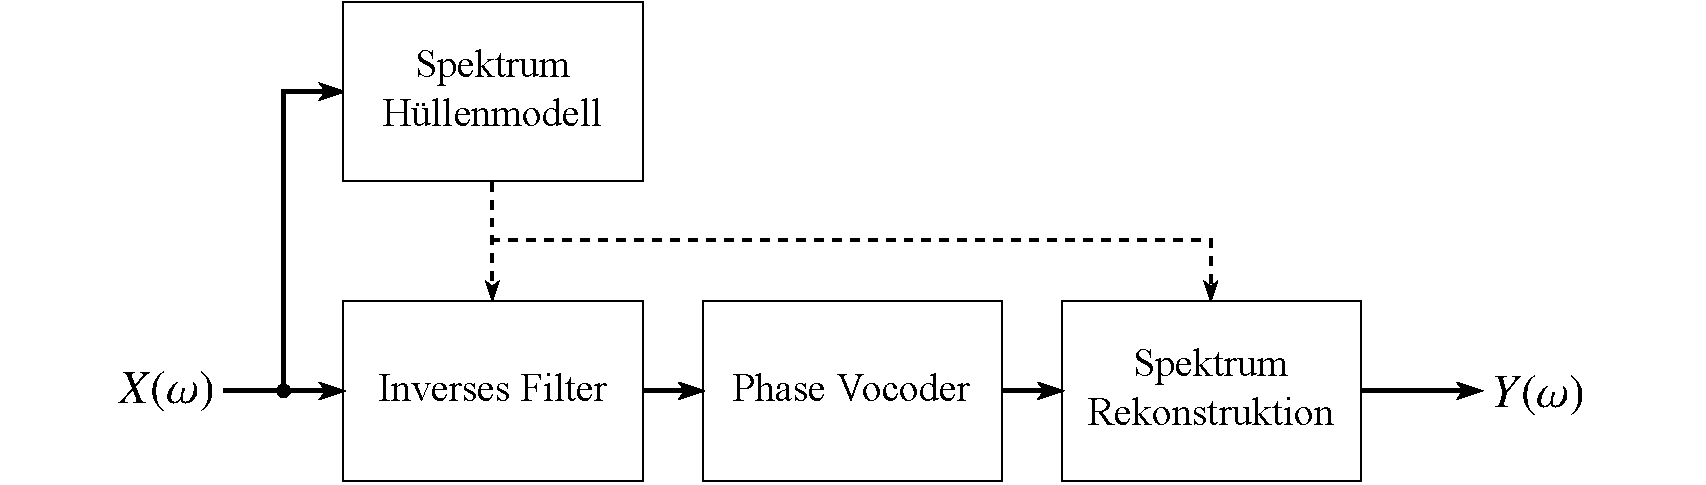
\includegraphics[width=\textwidth]{papers/autotune/images/Spektrum-Modellierung.pdf}
    \caption{Phase Vocoder mit Spektrum-Modellierung}
    \label{autotune:fig:pitchShiftingSpektrumModellierung}
\end{figure}
Als erstes wird die Umhüllende des Spektrums geschätzt.
Diese kann beispielsweise als All-Pol Modell modeliert werden.
Anschliessend wird mittels inversem Filter das Amplitudenspektrum normalisiert (flattening), ausgedrückt als
\begin{equation}
    X_{\text{flat}}(\omega)
    =
    X(\omega) \cdot \frac{1}{\hat{E}_x(\omega)} \;.
\end{equation}
Dabei ist $\hat{E}_x(\omega)$ die geschätzte Umhüllende des Spektrums.
In einem nächsten Schritt wird das Frequenzspektrum skalliert um die gewünschte Tonhöhe zu erreichen.
Zum Schluss folgt die Rekonstruktion der Spektrumumhüllenden mittels zuvor geschätztem All-Pol Modell.
Das resultierende, formantenerhaltende Spektrum ist somit
\begin{equation}
    Y(\omega)
    =
    X_{\text{flat}}(\omega \cdot R) \cdot \hat{E}_x(\omega) \;.
\end{equation}
In Abbildung \ref{autotune:fig:formantenErhaltung} ist der Unterschied zwischen der Spektrum Manipulation mit und ohne Formantenerhaltung dargestellt.
\begin{figure}
    \centering
    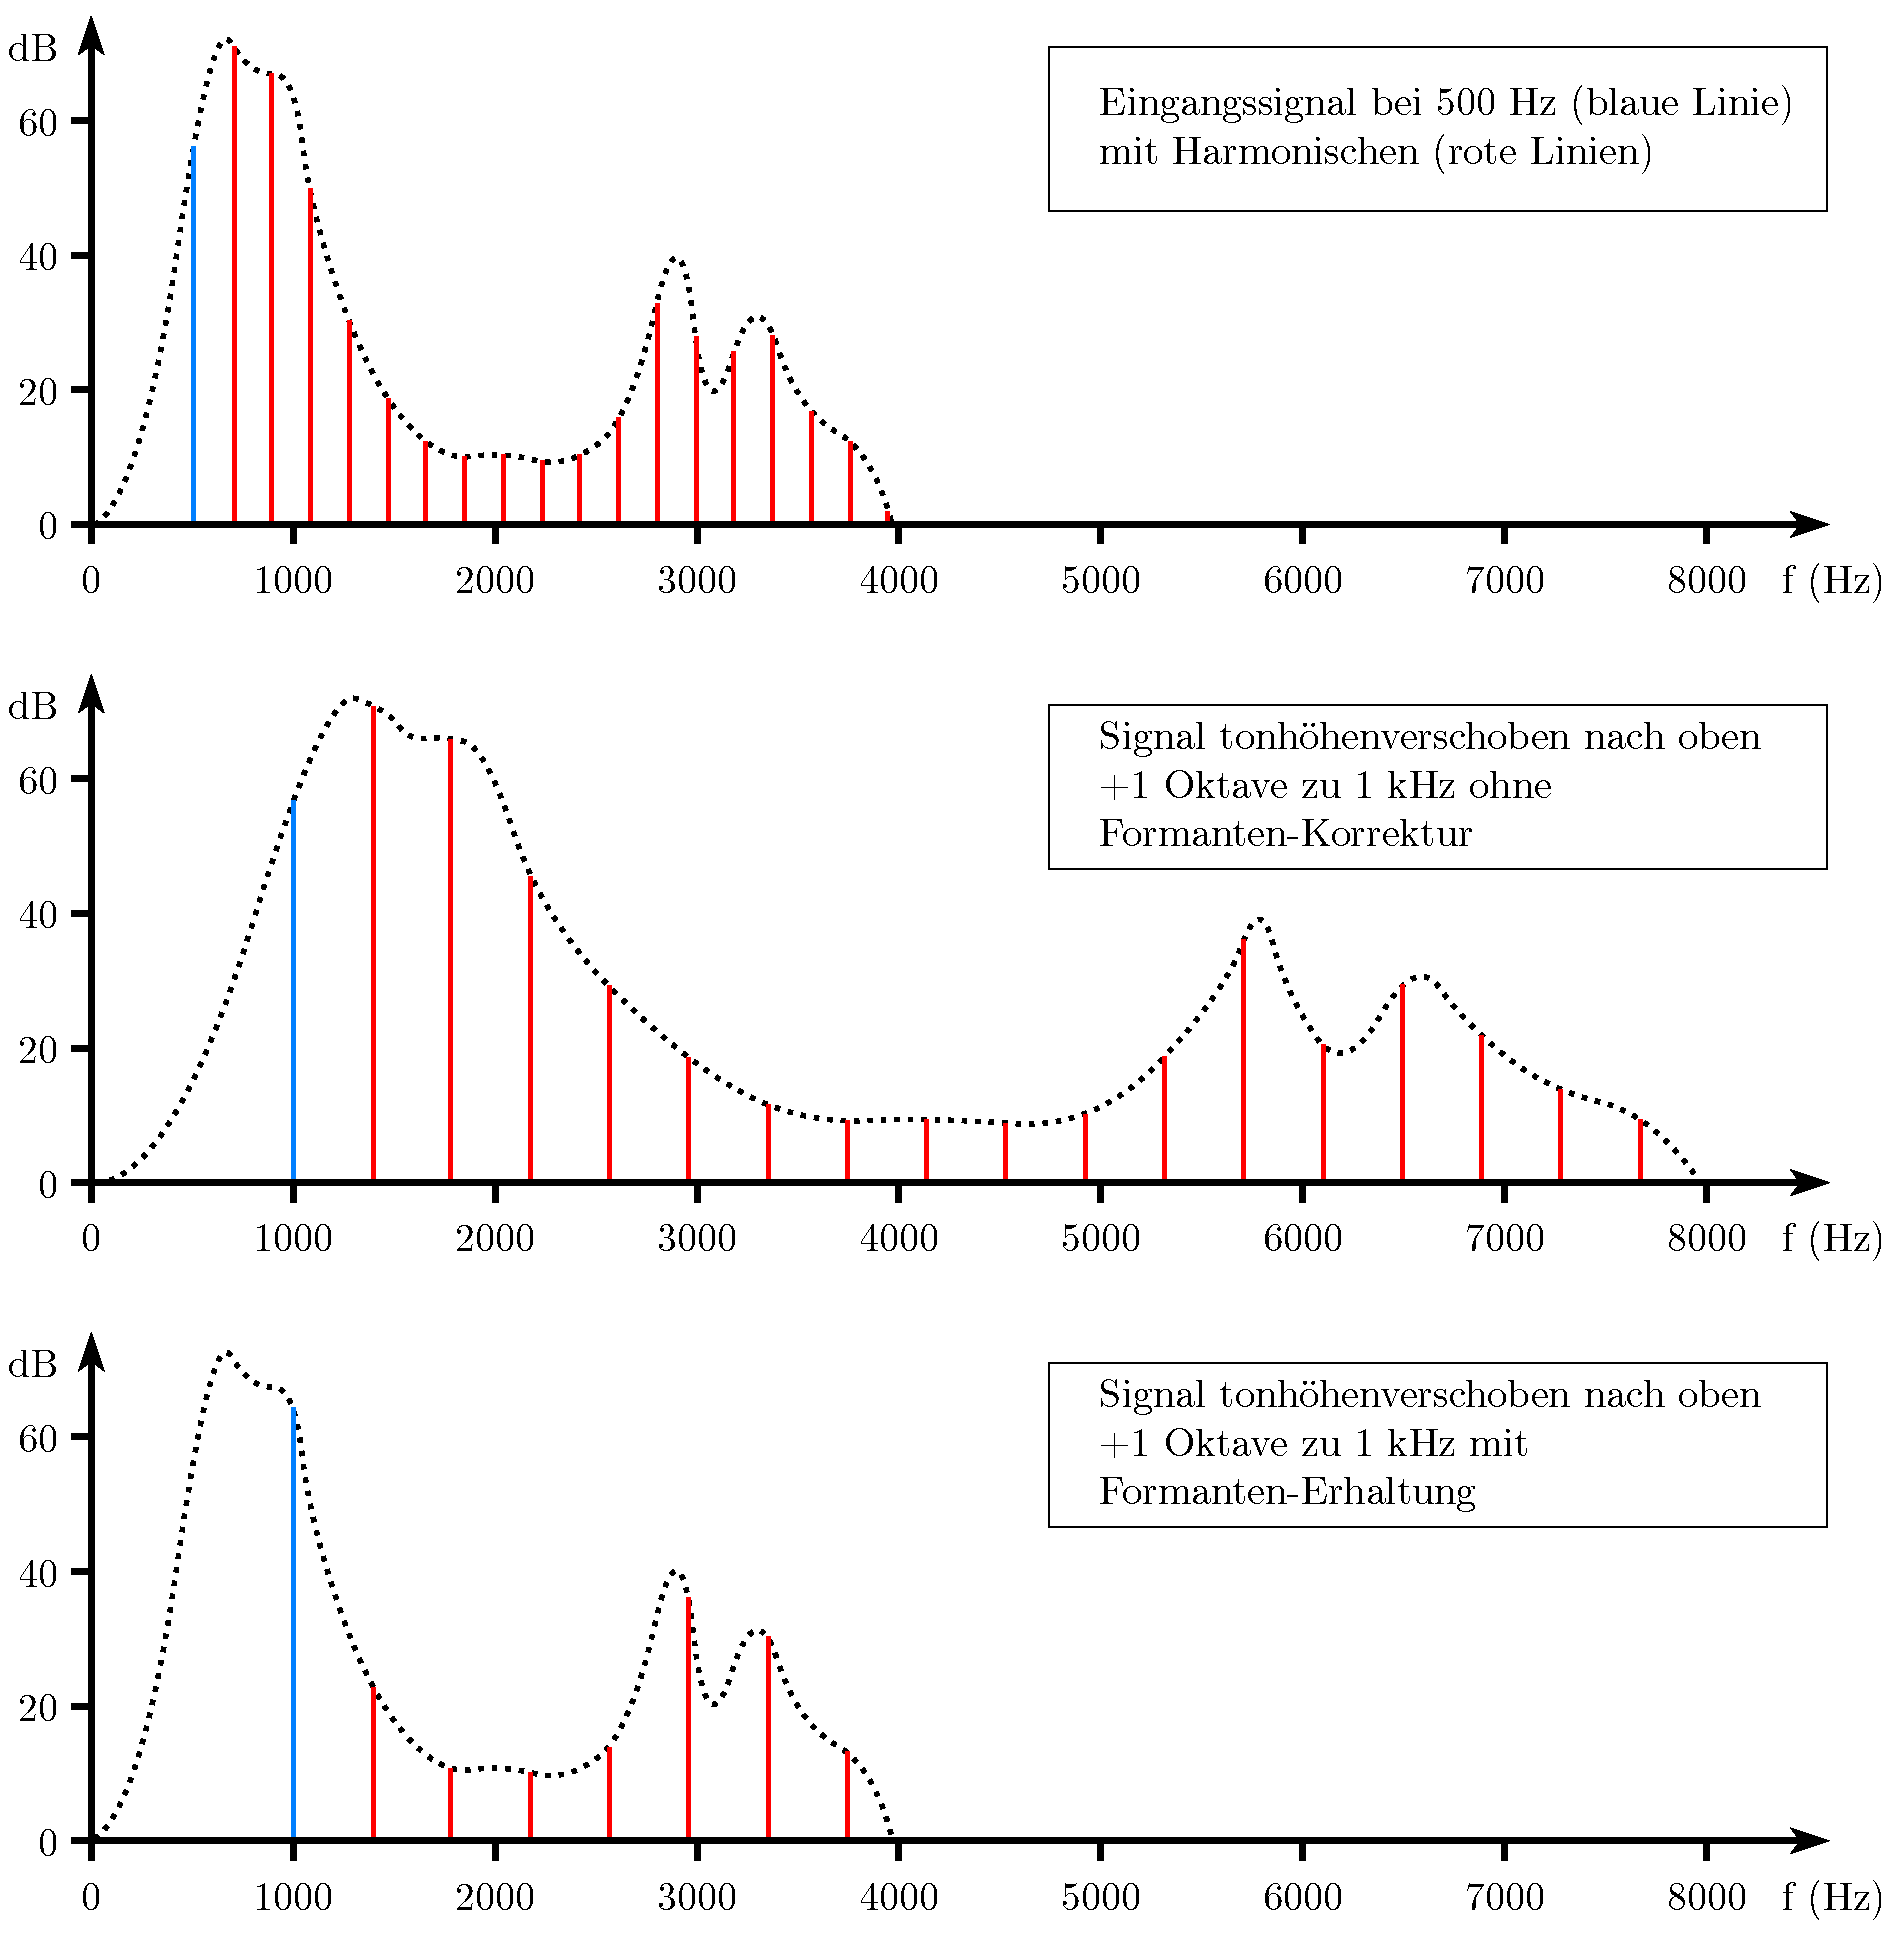
\includegraphics[width=0.95\textwidth]{papers/autotune/images/Formanten-Erhaltung.pdf}
    \caption{Spektrum Manipulation mit und ohne Formantenerhaltung}
    \label{autotune:fig:formantenErhaltung}
\end{figure}

% TODO: Add audio example pitch shifting with and without formant preservation


\subsection{Fensterrekonstruktion
\label{autotune:subsection:fensterRekonstruktion}}
Die Phasenrekonstruktion ist ein wichtiger Bestandteil des Phase Vocoders.
Ziel ist es die Phasensprünge zwischen den Fenstern zu minimieren.
In der Praxis kann dies jedoch nur näherungsweise erfolgen.
Das grundlegende Konzept kann gut anhand eines grafischen Beispiels (Abbildung \ref{autotune:fig:phaseReconstruction}) gezeigt werden.
\begin{figure}
    \centering
    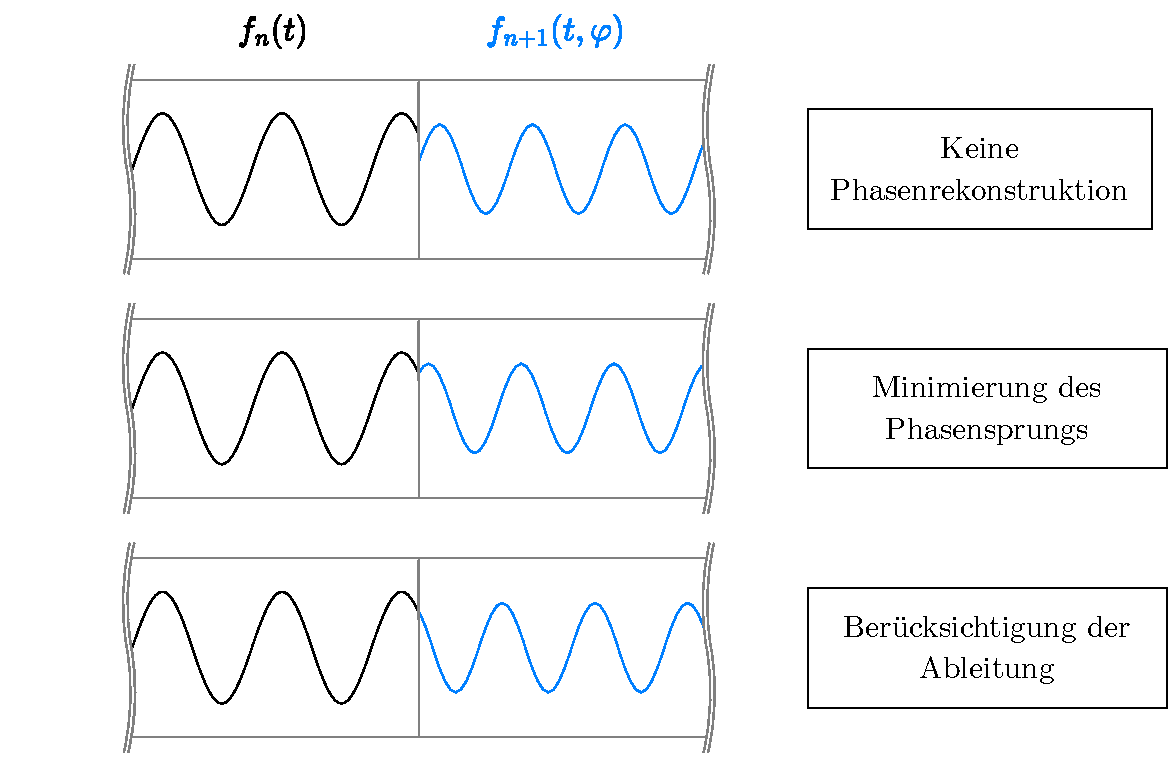
\includegraphics[width=0.8\textwidth]{papers/autotune/images/Fenster-Rekonstruktion.pdf}
    \caption{Fenster Rekonstruktion mit und ohne Berücksichtigung der Phasen}
    \label{autotune:fig:phaseReconstruction}
\end{figure}

Gegeben seien die Fenster als Funtionen $f_n(t)$ und $f_{n+1}(t, \varphi)$.
Sie sind das Resultat der inversen Short-Time-Fouriertransformation (ISTFT) des manipulierten Spektrums,
ausgedrückt als
\begin{equation}
    \begin{aligned}
        f_n(t)
        &=
        \sum_{\omega} X(n, \omega) e^{j\omega t} w(t - n) \\
        f_{n+1}(t, \varphi)
        &=
        \sum_{\omega} X(n+1, \omega) e^{j(\omega t + \varphi)} w(t - (n+1)) \;.
    \end{aligned}
\end{equation}
Es gilt nun also die Phasenverschiebung $\varphi$ des nachfolgenden Fensters $f_{n+1}$ so zu wählen,
dass die Differenz zwischen dem vorherigen Fenster $f_n$ zum Zeitpunkt $t_0$ (Überlappungszeitpunkt) minimal wird.
Des weiteren gilt es zu beachten, dass zusätzlich auch die Vorzeichen der Ableitungen $\dot{f}_n$ und $\dot{f}_{n+1}$ übereinstimmen müssen,
um einen monotomen Übergang zwischen den Fenstern zu gewährleisten.
Das Optimierungsproblem kann wie folgt formuliert werden:
\begin{equation}
    \begin{aligned}
        \underset{\varphi \; \in \; \mathbb{R}}{\text{minimize}}
        & \quad
        \Delta f(t=t_0, \varphi) = |f_n(t) - f_{n + 1}(t, \varphi)| \\
        \text{subject to}
        & \quad
        \text{sign}(\dot{f}_n(t_0)) \stackrel{!}{=} \text{sign}(\dot{f}_{n + 1}(t_0, \varphi)) \\
        & \quad
        0 \leq \varphi < 2\pi \;.
    \end{aligned}
\end{equation}
In der Praxis wird oft mit einem Überlappungsfaktor zwischen den Fenstern gearbeitet, der die Phasensprünge weiter reduziert (Stichwort Overlap-Add).
Der Überlappungsfaktor bestimmt, wie viel eines Fensters mit dem vorherigen und nachfolgenden Fenster überlappt.
Ein Überlappungsfaktor von 50\% bedeutet beispielsweise, dass die Fenster zur Hälfte überlappen.
Bei guter Umsetzung dieses Verfahren kann die Qualität der rekonstruierten Audiosignale stark verbessert werden.
Ansonsten können hörbare Artefakte entstehen, welche sich beispielsweise als \glqq metallischer Klang\grqq\ oder erhöhtes Rauschen äussern.

% TODO: Add audio examples of baddly and well reconstructed frames

%
% 04_Fazit.tex
%
% (c) 2023 Florian Baumgartner, OST Ostschweizer Fachhochschule
%
% !TEX root = ../../buch.tex
% !TEX encoding = UTF-8
%
\section{Fazit
\label{autotune:section:fazit}}
\rhead{Fazit}
Die mathematischen Prinzipien hinter Auto-Tune, insbesondere die Fourier-Transformation und die Phasenrekonstruktion,
sind Schlüsselelemente für die Genauigkeit und Qualität des endgültigen Ausgangssignals.
Durch fortlaufende Verbesserungen und Anpassungen dieser Algorithmen ist es möglich, immer natürlicher klingende Korrekturen zu erzielen.

Insgesamt zeigt das Thema Auto-Tune eindrucksvoll, wie mathematische Konzepte wie die der harmonischen Analysis direkt in praktischen Anwendungen wie der Musikproduktion eingesetzt werden können.
Die kontinuierliche Weiterentwicklung dieser Techniken bietet nicht nur Möglichkeiten zur Verbesserung der künstlerischen Ausdrucksformen,
sondern liefert auch wertvolle Einblicke in die Komplexität und Vielseitigkeit der digitalen Signalverarbeitung.


\printbibliography[heading=subbibliography]
\end{refsection}
